\documentclass{article}[11pt]

\usepackage{amsmath}
\usepackage{booktabs}
\usepackage{hyperref}
\usepackage{setspace}
\usepackage{soul}
\usepackage[margin=1.2in]{geometry}
\usepackage{natbib}
\usepackage{pgf,tikz}
\usepackage{pgfplots}

\bibliographystyle{abbrvnat}
\bibpunct{(}{)}{;}{a}{,}{,}


\setlength{\parskip}{5mm}
\setlength{\parindent}{0cm}

\usetikzlibrary{decorations}
\usetikzlibrary{shapes,arrows}
\tikzstyle{block} = [rectangle, draw, fill=blue!20, 
    text width=6em, text centered, rounded corners, minimum height=4em]
\tikzstyle{block2} = [rectangle, draw, 
    text width=8em, text centered, minimum height=2em]
\tikzstyle{block3} = [rectangle, draw, 
    text width=6em, text centered, minimum height=2em]
\tikzstyle{line} = [draw, -latex']
\tikzstyle{line1} = [draw]


\title{GETS: A General-to-Specific Algorithm in Stata}
\author{Damian Clarke\thanks{\href{mailto:damian.clarke@economics.ox.ac.uk}{damian.clarke@economics.ox.ac.uk}}}
\date{\today}

\begin{document}

\maketitle
\begin{abstract}
 This article describes the application of a well known model fitting algorithm to Stata: general-to-specific
 (GETS) modelling.  It discusses a number of empirical issues in GETS modelling, specifically how such an
 algorithm can be applied to models based upon cross-sectional, time-series and panel data.  A command is then
 presented, written in Stata and Mata, which implements this algorithm for various data types in a flexible way.
 This command, \texttt{gets}, is then illustrated using real empirical data from applied studies of GETS modelling 
 and with Monte Carlo simulation.  It is shown to perform as empirically predicted, and to have good size and power 
 (or gauge and potency) under simulation.
\end{abstract}

\begin{spacing}{1.2}
\section{Introduction}
General-to-specific modelling (hereafter GETS) is an important class of model selection in econometrics.
In comparison to 

This can in some sense be though of as data-based model selection.  While this may seem concerning to
economists typically concerned with `data-mining', the LSE-school of modelling, led perhaps by Hendry 
and co-authors suggests that this is not the case.  Rather than assuming that the econometrician perfectly
understands the true data generating process (DGP), a GETS approach espouses the formation of some general 
unrestricted model (or GUM) based upon theory which includes a 


\section{Algorithm Description}
The search algorithm undertaken by \texttt{gets} depends upon the model type and GUM specified by the
user.  Whether the underlying model is based upon cross-sectional, time-series, or panel data determines
the set of initial tests (``the battery'') and the set of subsequent tests run at each stage of the search
path.  In what follows we discuss the general search algorithm followed for every model, delaying discussion
of specific tests until the corresponding subsections for cross-sectional, time-series, and panel models
respectively.

In defining the search algorithm, we follow that described in \citet{HooverPerez1999}, and in appendix A of
\citet{HooverPerez2004}.  \citet{HooverPerez1999} is generally considered to be an important starting point
in the description of a computational general-to-specific modelling process (see for example 
\citet{Camposetal2005}).  The algorithm takes the following form:

\begin{enumerate}
 \item The user specifies their proposed GUM, and indicates to Stata the relevant data, if necessary using
 \emph{if} and \emph{in} specifiers.
 \item 90 percent of the full sample is retained, while the remaining 10 percent is set aside for out-of-sample 
 testing.  On this 90 percent sample the battery of tests is run at the nominal size.\footnote{In subsections 
 \ref{sscn:Acs}--\ref{sscn:Axt} we discuss the specific nature of these tests, and the determination of the
 in-sample and out-of-sample observations}.  If one of these tests is failed, it is eliminated from the battery
 in the following steps of the search path (for the current replication).  If more than one of these tests is 
 failed by the GUM, the user is instructed that the GUM is likely a poor representation of the true model, and
 an alternative general model is requested.\footnote{As in all terminal decisions, the user is able to override
 this decision and continue with their proposed GUM if so desired.}
 \item Each variable in the general model is ranked by the size of their \emph{t}-statistic and the algorithm 
 then follows \emph{n} (by default 5) search paths.  The first search path is initiated by eliminating the lowest
 (insignificant) variable from the GUM.  The second follows the same process, but rather than eliminating the
 lowest, eliminates the second lowest.  This process is followed until reaching the $n$\textsuperscript{th} search 
 path which eliminates the $n$\textsuperscript{th} lowest variable.  For each search path, the current specification
 then includes all remaining variables, and this specification is estimated.
 \item The current specification is then subjected to the full battery of tests, along with an \emph{F}-test to
 determine if the current specification is a valid restriction of the GUM.  If any of these tests are failed the
 current search path is abandoned, and the algorithm jumps to the subsequent search path.
 \item If the current specification passes the above tests, the variables in the current specification are once
 again ordered by the size of their \emph{t}-statistic, and the next lowest variable is eliminated.  This then
 becomes a potential current specification, which is subjected to the battery of tests.  If any of these 
 tests are failed, the model reverts to the previous current specification, and the second lowest (insignificant) 
 variable is eliminated.  Such a process is followed until a variable is successfully eliminated, or all insignificant 
 variables have been attempted.  If an insignificant variable is eliminated, stage 5 is then restarted with the
 current specification.  This process is then followed iteratively, until either all insignificant variables
 have been eliminated, or no more variables can be successfully removed.
 \item Once no further variables can be eliminated, a potential terminal specification is reached.  This 
 specification is estimated on the full sample of data.  If all variables are significant it is accepted as the 
 terminal specification.  If any insignificant variables remain, these are eliminated as a group and the new 
 terminal specification is subjected to the battery of tests.  If it passes these tests it is the terminal 
 specification, and if not, the previous terminal specification is accepted.
 \item Each of the $n$ terminal specifications is compared, and if these are different, the final specification
 is determined using an information criterion or encompassing (see the related discussion in sections \ref{sscn:Acs}
 -\ref{sscn:Axt}).
\end{enumerate}

\subsection{Cross-sectional Models}
\label{sscn:Acs}
Cross sectional models are subjected to an initial battery of five tests.  These are a Doornik-Hansen test for normality
of errors, the \citet{BreuschPagan1979} test for homoscedasticity of errors\footnote{This test is not run if the the model 
estimated is robust to this type of misspecification.}, the RESET test for the linearity of coefficients \citep{Ramsey1969}
and an in-sample and out-of-sample stability \emph{F}-test.  These two final tests consist of a comparison of regressions
of each subsample to estimation results for the full sample: in the in-sample case the two subsamples are made up of two
halves of the full sample, while in the out-of-sample test this is a comparison between the 90 percent and ten percent samples.
These tests are analogous to \citet{Chow1960} tests.

The determination of the final model using OLS with cross-sectional data is via information criteria.  For each of the
$n$ potential terminal specifications, a regression is run and the Bayesian Information Criterion (BIC) is calculated.
That terminal specification which has the lowest BIC is determined to be the final specification.
\subsection{Time-Series Models}
\label{sscn:Ats}
In time series models, an additional test in included in the battery discussed above.  Along with Doornik-Hansen, Breusch-%
Pagan, RESET, and in- and out-of-sample Chow tests, a test is run for autocorrelated conditional heteroscedasticity (or ARCH) 
up to the second order \citep{Engle1982}.  In order to partition the sample into `in-sample' and `out-of-sample', the 
final 10\% of observations are initially discarded to be used in out of sample tests.  These are (as in all cases) returned
to the sample in the calculation of the final model, and in choosing between various terminal specifications, a BIC is once
again used.


\subsection{Panel-data Models}
\label{sscn:Axt}
\citet{Drukker2003} \citet{Wooldridge2002} \citet{BreuschPagan1980}

\section{The gets command}
\subsection{Syntax}
\texttt{gets} \emph{yvar} \emph{xvars} [\emph{if}] [\emph{in}] [\emph{weight}] [, \texttt{vce}(\emph{vcetype}) \texttt{xt}(\texttt{re|fe|be}) \texttt{ts}(\emph{regcmd}) \texttt{\ul{nodiag}nostic} \texttt{tlimit}(\emph{\#})
\texttt{\ul{nums}earch}(\#) \texttt{\ul{nopart}ition} \texttt{noserial} \texttt{verbose} ]

\subsection{Options}
\texttt{vce}(\emph{vcetype}) \emph{vcetype} determines the type of standard error reported in the
estimated regression model, and allows standard errors that are robust to certain types of 
misspecification.  \emph{vcetype} may be robust, cluster clustvar, bootstrap, or jackknife.

\texttt{xt}(\texttt{re|fe|be}) specifies that the model is based on panel data.  The user must specify
whether they wish to estimate a random-effects (RE), fixed-effects (FE), or between-effects (BE) model.  
By default \texttt{re} is assumed.  \texttt{xtset} must be specified prior to using this option.

\texttt{ts} specifies that the model is based on time-series data.  \texttt{tsset} must be specified 
prior to using this option, and if specified, time-series operators may be used.

\texttt{\ul{nodiag}nostic} turns off the initial diagnostic tests for model misspecification.  This
should be used with caution.

\texttt{tlimit}(\emph{\#}) sets the critical t-value above which variables are considered as important 
in the terminal specification.  By default this is a value of 1.96.

\texttt{\ul{nums}earch} defines the number of search paths to follow in the model.  If not specified, 5
search paths are followed.  If a large dataset is used, fewer search paths may be preferred.

\texttt{\ul{nopart}ition} uses the full sample of data in all search paths, and does not engage in
out of sample testing.

\texttt{noserial} requests that no serial correlation test is performed if panel data is being used.

\texttt{verbose} requests full program output of each search path explored.

\subsection{Returned Objects}
\texttt{gets} is an eclass program, and returns a number of elements in the e list.  It returns the
BIC of the preferred model, along with the list of variables preferred by the model, and---in the 
case that the final model is not encompassing---a full list of variables which are determined as 
important in \emph{any} terminal specification.  These are available as \texttt{e(fit)}, \texttt{e(gets)},
and \texttt{e(gets\_all)} respectively.  The full ereturn list which includes regression results for
the terminal specification is available as \texttt{ereturn list}.

\section{Performance in Monte Carlo Simulation}

\section{Conclusion}

\newpage
\bibliography{refs.bib}

\end{spacing}
\end{document}














\section*{Appendices}
\appendix
\section{Diagramatical Representation of Search Algorithm}
\scalebox{1.2}{
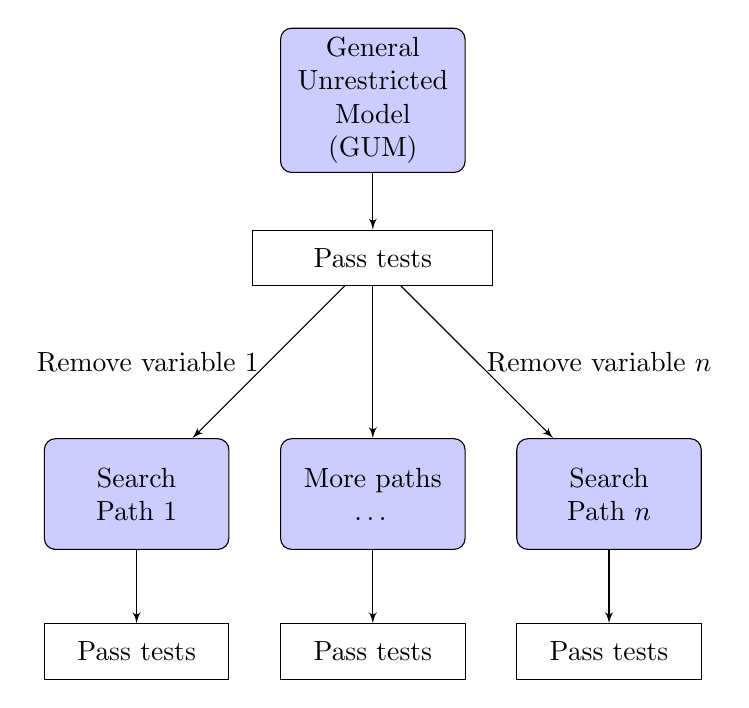
\begin{tikzpicture}[node distance = 3.5cm, auto]
    % Place nodes
    \node [block] (GUM) {General Unrestricted Model (GUM)};
    \node [block2, below of=GUM, node distance=2cm] (test1) {Pass tests};
    \node [block, below of=test1, node distance=3cm] (SP2) {More paths \\ \ldots};
    \node [block, left of=SP2, node distance=3cm] (SP1) {Search Path 1};
    \node [block, right of=SP2, node distance=3cm] (SPn) {Search Path $n$};    
    \node [block3, below of=SP1, node distance=2cm] (test2a) {Pass tests};
    \node [block3, below of=SP2, node distance=2cm] (test2b) {Pass tests};
    \node [block3, below of=SPn, node distance=2cm] (test2c) {Pass tests};
    
    
    
    
    
 %   \node [block, below of=SP2] (CR) {Couple's Recode (CR)};
 %   \node [block, left of=CR, node distance=4cm] (IR) {Individual Women's Recode (IR)};
 %   \node [block, right of=CR, node distance=4cm] (MR) {Male Recode (MR)};    
 %   \node [block, below of=IR] (KR) {Children's Recode (KR)};
 %   \node [block, below of=CR] (BR) {Birth Recode (BR)};
 %   \node [below of=CR, node distance=1.7cm] (link) {};    
 %   \node [below of=CR, node distance=45.5pt] (link1) {};    

    % Draw edges
    \path [line] (GUM) --node [right] {} (test1);
    \path [line] (test1) --node [left] {Remove variable 1} (SP1);
    \path [line] (test1) --node [left] {} (SP2);
    \path [line] (test1) --node [right] {Remove variable $n$} (SPn);
    \path [line] (SP1) --node [right] {} (test2a); 
    \path [line] (SP2) --node [right] {} (test2b); 
    \path [line] (SPn) --node [right] {} (test2c);     
    %    \path [line] (SP2) -| node [above]{\textbf{1:m}}(IR);
%    \path [line] (SP2) -| node [above]{\textbf{1:m}}(MR);
 %   \path [line,dashed] (IR) -- node [above]{\textbf{1:m}}(CR);
 %   \path [line,dashed] (MR) -- node [above]{\textbf{1:m}}(CR);    
 %   \path [line] (IR) --node [left] {\textbf{1:m}} (KR);
 %   \path [line1] (IR) |- (link);
 %   \hspace{-3.5pt}\path [line] (link1) -- node [right] {\textbf{1:m}}(BR);

\end{tikzpicture}
}

